\documentclass{beamer}
\usepackage{etex}

%\useoutertheme[glossy]{wuerzburg}
\useinnertheme[shadow,outline]{chamfered}
%\usecolortheme{shark}
\usecolortheme{beaver}
\beamertemplatenavigationsymbolsempty

\usefonttheme{professionalfonts}
\let\digamma\relax
\usepackage[scale=0.85,stdmathitalics=true,romanfamily=casual]{lucimatx}
\usefonttheme[stillsansseriftext]{serif}



\usepackage{fancyvrb}

%% Fancy syntax coloring via pygments
\usepackage{minted}
\definecolor{bg}{rgb}{0.95,0.95,0.95}
\usemintedstyle{borland}


\newenvironment{Rcode}
{\VerbatimEnvironment
 \begin{minted}[fontsize=\scriptsize,baselinestretch=1]{r}}%
{\end{minted}}

\newenvironment{Pcode}
{\VerbatimEnvironment
 \begin{minted}[fontsize=\scriptsize,baselinestretch=1]{python}}%
{\end{minted}}

\newenvironment{Code}[1]
{\VerbatimEnvironment
 \begin{minted}[fontsize=\scriptsize,baselinestretch=1]{#1}}%
{\end{minted}}


\usepackage{textfit} % commands \scaletoheight{height}{text} and \scaletowidth{width}{text}

\usepackage{tikz}

\usepackage{tcolorbox}

\newtheorem{Alert}{Alert}
\newtheorem{Highlight}{Highlight}

\newcommand{\Species}[1]{{\rmfamily \itshape #1}}
\newcommand{\Real}{\ensuremath{\mathbb{R}}}
\newcommand{\RealN}{\ensuremath{\mathbb{R}^n}}
\newcommand{\RealP}{\ensuremath{\mathbb{R}^p}}
\newcommand{\Mtx}[1]{\ensuremath{\mathbf{#1}}}
\newcommand{\Inv}[1]{\ensuremath{#1^{-1}}}
\newcommand{\InvMtx}[1]{\ensuremath{\mathbf{#1}^{-1}}}
\newcommand{\Red}[1]{\textcolor{red}{#1}}
\newcommand{\PsInv}[1]{\ensuremath{\mathbf{#1}^{+}}}

\usepackage{booktabs}



% --- Macro \xvec
% From a tex.stackexchange.com answer by Todd Lehman
% http://tex.stackexchange.com/questions/44017/dot-notation-for-derivative-of-a-vector
\makeatletter
\newlength\xvec@height%
\newlength\xvec@depth%
\newlength\xvec@width%
\newcommand{\xvec}[2][]{%
  \ifmmode%
    \settoheight{\xvec@height}{$#2$}%
    \settodepth{\xvec@depth}{$#2$}%
    \settowidth{\xvec@width}{$#2$}%
  \else%
    \settoheight{\xvec@height}{#2}%
    \settodepth{\xvec@depth}{#2}%
    \settowidth{\xvec@width}{#2}%
  \fi%
  \def\xvec@arg{#1}%
  \def\xvec@dd{:}%
  \def\xvec@d{.}%
  \raisebox{.2ex}{\raisebox{\xvec@height}{\rlap{%
    \kern.05em%  (Because left edge of drawing is at .05em)
    \begin{tikzpicture}[scale=1]
    \pgfsetroundcap
    \draw (.05em,0)--(\xvec@width-.05em,0);
    \draw (\xvec@width-.05em,0)--(\xvec@width-.15em, .075em);
    \draw (\xvec@width-.05em,0)--(\xvec@width-.15em,-.075em);
    \ifx\xvec@arg\xvec@d%
      \fill(\xvec@width*.45,.5ex) circle (.5pt);%
    \else\ifx\xvec@arg\xvec@dd%
      \fill(\xvec@width*.30,.5ex) circle (.5pt);%
      \fill(\xvec@width*.65,.5ex) circle (.5pt);%
    \fi\fi%
    \end{tikzpicture}%
  }}}%
  #2%
}
\makeatother

% --- Override \vec with an invocation of \xvec.
\let\stdvec\vec
\renewcommand{\vec}[1]{\xvec[]{#1}}
% --- Define \dvec and \ddvec for dotted and double-dotted vectors.
\newcommand{\dvec}[1]{\xvec[.]{#1}}
\newcommand{\ddvec}[1]{\xvec[:]{#1}}


\usepackage{pifont}
\newcommand{\weblink}{\ding{43}}  % hand with pointing finger

\definecolor{links}{HTML}{2A1B81}
\hypersetup{colorlinks,linkcolor=,urlcolor=magenta}

\usepackage{tikz}

\usepackage[inline]{asymptote}
\usepackage{attachfile2}
\usepackage{asyfig}




%===========================================================
% Title Info
\title{Scientific Computing for Biologists}
\subtitle{Linear Algebra Review I} % (optional)

\author{Instructor: Paul M. Magwene}


\date{09 September 2014}

\begin{document}
%===========================================================
\begin{frame}
\titlepage
\end{frame}

%===========================================================
\begin{frame}
  \frametitle{Overview of Lecture}
  
\begin{itemize}
        \item ANOVA as bivariate regression
        \item Partial correlation
	\item Introduction to Matrices
		\begin{itemize}
			\item Matrices as collections of vectors
			\item Special matrices
		\end{itemize}
		\item Matrix operations
		\begin{itemize}
			\item Matrix addition, subtraction
			\item Matrix multiplication
		  \item Transpose			
		  \item More special matrices		  
		\end{itemize}		
	  \item Matrices as linear transformations		
		\item Linear dependence/independence
		\item Matrix inverses		
		\item Solving simultaneous linear equations
\end{itemize}

\end{frame}
%===========================================================

% %===========================================================
% \begin{frame}
%   \frametitle{Hands-on Session}
% 		\begin{itemize}
%     \item Matrices in R
% 		\item Standard statistics as matrix operations
%         \begin{itemize}
%         	\item Mean vector
%         	\item Deviates matrix
%         	\item Covariance matrix
%         	\item Correlation matrix
%         	\item Concentration matrix / Partial corelations
%         	\item Euclidean distance matrix		  
%         \end{itemize}
% 		  
% 	\item Graphical plots for multivariate data in R
%         \begin{itemize}
%         	\item Scatter plot matrix
%             \item 3D scatter plots
%             \item Color grid plots
%         \end{itemize}
% 
%     \item Tools for reshaping, aggregating, and summarizing data in R
%         \begin{itemize}
%             \item reshape2 package
%         \end{itemize}
%     \end{itemize}
% 
% \end{frame}		
%===========================================================

%===========================================================
\begin{frame}
  \frametitle{Geometry of Bivariate Regression}

Geometric interpretation of regression as projection:

\begin{center}

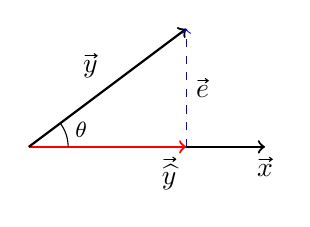
\begin{tikzpicture}[x=0.5cm, y=0.5cm]

\draw[thick,->] (0,0) -- (6,0);
\draw (6,0) node[below] {$\vec{x} $};

\draw[thick,red,->] (0,0) -- (4,0);
\draw (4,0) node[below left] {$\vec{\widehat{y}}$};

\draw[thick,->] (0,0) -- (4,3);
\draw (2,1.5) node[above left] {$\vec{y}$};

\draw[dashed,blue,->] (4,0) -- (4,3);
\draw (4,1.5) node[right] {$\vec{e}$};

\draw (0,0) +(0:0.5cm) arc (0:37:0.5cm);
\path (0,0) ++(18:0.7cm) node[font=\footnotesize] {$\theta$};

\end{tikzpicture}

\[
\vec{\widehat{y}} = b\vec{x}
\]
\begin{equation}
b = \frac{\vec{x} \cdot \vec{y}}{\vec{x} \cdot \vec{x}}
\end{equation}

\end{center}

\end{frame}
%===========================================================



%===========================================================
\begin{frame}
  \frametitle{Two-group ANOVA as Regression}

We can also use a geometric perspective to test whether the mean of a variable differs between two groups of subjects.

\begin{itemize}
\item Setup a `dummy variable' as the predictor $X_g$.   We assign all subjects in group 1 the value 1 and all subjects in group 2 the value -1 on the dummy variable.  We then regress the variable of interest, $Y$, on $X_g$.

\end{itemize}
%
$$
\Mtx{y} = \Mtx{X}_g\Mtx{b} + \Mtx{e}
$$
%
\begin{figure}
{\centering 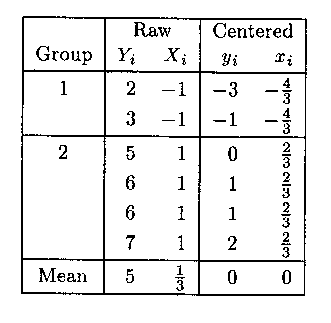
\includegraphics[height=1.5in]{anova-2group-table.pdf}}
\end{figure}


\end{frame}
%===========================================================


%===========================================================
\begin{frame}
  \frametitle{Two-group ANOVA as Regression, cont}

\begin{itemize}

\item When the means are different in the two groups, $X_g$ will be a good predictor of the variable of interest, hence $\vec{y}$ and $\vec{x_g}$ will have a small angle between them.

\item When the means in the two groups are similar, the dummy variable will not be a good predictor.  Hence the angle between $\vec{y}$ and $\vec{x_g}$ will be large.

\end{itemize}

\begin{center}

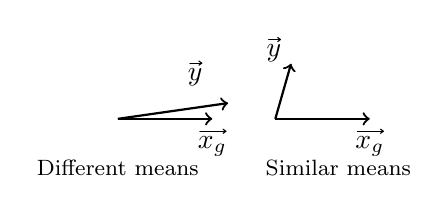
\begin{tikzpicture}[x=0.2cm, y=0.2cm]

% different means
\draw[thick,->] (-10,0) -- (-4,0);
\draw (-4,0) node[below] {$\vec{x_g}$};

\draw[thick,->] (-10,0) -- (-3,1);
\draw (-4,1.5) node[above left] {$\vec{y}$};
\draw (-10,-2) node[below,font=\footnotesize] {Different means};

% Similar means
\draw[thick,->] (0,0) -- (6,0);
\draw (6,0) node[below] {$\vec{x_g}$};

\draw[thick,->] (0,0) -- (1,3.5);
\draw (1,3) node[above left] {$\vec{y}$};
\draw (4,-2) node[below,font=\footnotesize] {Similar means};

\end{tikzpicture}

\end{center}

\end{frame}
%===========================================================


%===========================================================
\begin{frame}
  \frametitle{Geometry of the Population Regression Model}


\begin{figure}
{\centering 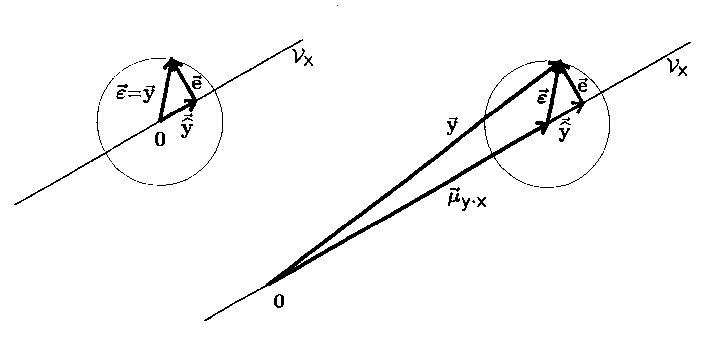
\includegraphics[height=2in]{regr-error-model2.pdf}}
\caption{\textbf{Left:} null hypothesis of no regression effects is true; \textbf{Right:} null model is false.}
\end{figure}

\begin{center}
\alert{Is my regression significant? $\implies$ Is $|\vec{\hat{y}}|^2$ large relative to $|\vec{e}|^2$?}
\end{center}

\end{frame}
%===========================================================

%===========================================================
\begin{frame}
  \frametitle{Comparing the Effect Space and the Error Space}

To compare the squared length of $|\vec{\hat{y}}|^2$ and $|\vec{e}|^2$ we divide them by the dimension of the subspaces in which they lie.
\begin{align*}
M(\vec{\hat{y}}) &= \frac{|\vec{\hat{y}}|^2} {\dim(\mathcal{V}_x)}   \\
M(\vec{e})       &= \frac{|\vec{e}|^2}{\dim(\mathcal{V}_e)}
\end{align*}

We compare these by defining a statistic, $F$:
\begin{align*}
  F = \frac{M(\vec{\hat{y}})}{M(\vec{e})} &= \frac{\dim(\mathcal{V}_e)|\vec{\hat{y}}|^2}
                                                  {\dim(\mathcal{V}_x)|\vec{e}|^2}\\
 &= \frac{(N-p-1)R^2}{p(1-R^2)}
\end{align*}

\alert{When null hypothesis is true, $F\approx 1$; when it is false, $F \gg 1$.}

\end{frame}
%===========================================================

% %===========================================================
% \begin{frame}
%   \frametitle{Two-group ANOVA as Regression}

% We can also use a geometric perspective to test whether the mean of a variable differs between two groups of subjects.

% \begin{itemize}
% \item Setup a `dummy variable' as the predictor $X_g$.   We assign all subjects in group 1 the value 1 and all subjects in group 2 the value -1 on the dummy variable.  We then regress the variable of interest, $Y$, on $X_g$.  

% \item When the means are different in the two groups, $X_g$ will be a good predictor of the variable of interest, hence $\vec{y}$ and $\vec{x_g}$ will have a small angle between them.

% \item When the means in the two groups are similar, the dummy variable will not be a good predictor.  Hence the angle between $\vec{y}$ and $\vec{x_g}$ will be large.

% \end{itemize}

% \begin{center}

% \begin{tikzpicture}[x=0.2cm, y=0.2cm]

% % different means
% \draw[thick,->] (-10,0) -- (-4,0);
% \draw (-4,0) node[below] {$\vec{x_g}$};

% \draw[thick,->] (-10,0) -- (-3,1);
% \draw (-4,1.5) node[above left] {$\vec{y}$};
% \draw (-10,-2) node[below,font=\footnotesize] {Different means};

% % Similar means
% \draw[thick,->] (0,0) -- (6,0);
% \draw (6,0) node[below] {$\vec{x_g}$};

% \draw[thick,->] (0,0) -- (1,3.5);
% \draw (1,3) node[above left] {$\vec{y}$};
% \draw (4,-2) node[below,font=\footnotesize] {Similar means};

% \end{tikzpicture}

% \end{center}

% \end{frame}
% %===========================================================


\begin{frame}
  \frametitle{Reminder: Correlation}

Last time we saw that correlation is a measure of association and is a function of the angle between two vectors (variables).

\begin{center}

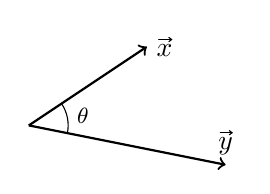
\begin{tikzpicture}[x=0.5cm, y=0.5cm]

\draw[thick,->] (0,0) -- (3,2);
\draw (3,2) node[right] {$\vec{x}$};

\draw[thick,->] (0,0) -- (5,-1);
\draw (5,-1) node[above] {$\vec{y}$};

\draw (0,0) +(-11:0.5cm) arc (-11:34:0.5cm);
\path (0,0) ++(10:0.7cm) node[font=\footnotesize] {$\theta$};

\end{tikzpicture}
\end{center}

\[
\mathsf{cor}(X,Y) = r_{XY} = \cos \theta = \frac{\vec{x} \cdot \vec{y}}{|\vec{x}||\vec{y}|}
\]


\alert{Q: Correlation is a pairwise measure. Can we extend this idea to more than two variables?}
\end{frame}


%===========================================================

\begin{frame}
  \frametitle{Partial Correlation}

{\small
The partial correlation of $\vec{x}$ and $\vec{y}$ given $\vec{z}$ is the correlation of $\vec{x}$ and $\vec{y}$ after we ``account for'' their joint association with $\vec{z}$.  

\medskip

What we mean by ``account for'' here is essentially `to factor out', by projecting $\vec{x}$ and $\vec{y}$ onto $\vec{z}$ and then calculating the correlation of the residual vectors.

}

\begin{center}
\asyinclude[width=7cm,inline=true]{partial-corr.asy}
%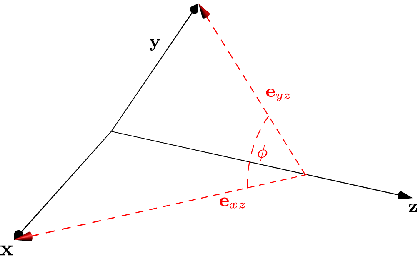
\includegraphics[width=6cm]{partial-corr.pdf}
\end{center}

\end{frame}



%===========================================================

\begin{frame}
  \frametitle{Geometry of Partial Correlation}

The partial correlation of $\vec{x}$ and $\vec{y}$ given $\vec{z}$ is equivalent to the correlation of the residuals after projecting $\vec{x}$ and $\vec{y}$ onto $\vec{z}$.

\begin{center}
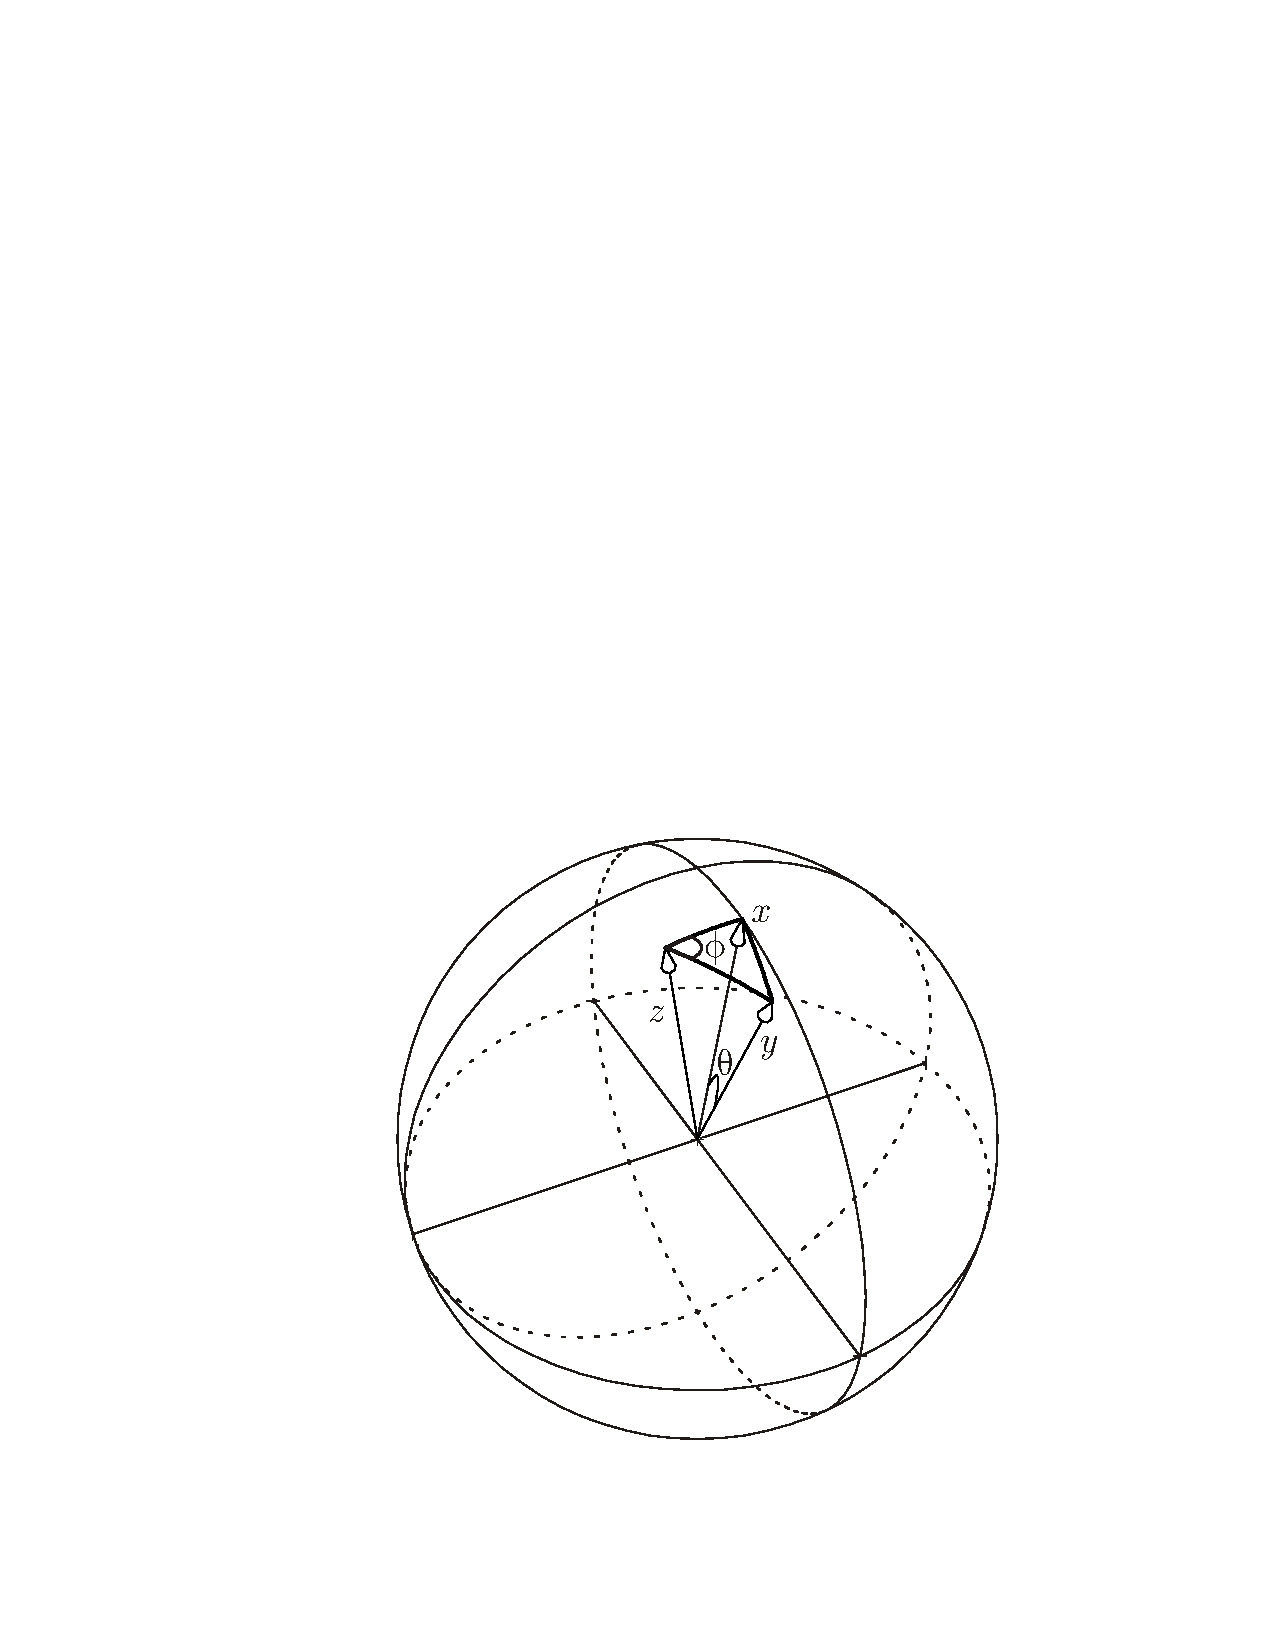
\includegraphics[width=4.5cm]{partial-corr-sphere.pdf}
\end{center}
\[
\mathsf{cor}(X,Y|Z) = r_{XY.Z} = \mathsf{cor}(\widehat{x}_{\bot z},\widehat{y}_{\bot z}) = \cos \phi
\]


\end{frame}

%===========================================================

\begin{frame}
  \frametitle{Algebra of Partial correlation}

Algebraicly, one can calculate the partial correlation between $X$ and $Y$ given $Z$ as:

\[
\mathsf{cor}(X,Y|Z) = r_{XY.Z} = \frac{r_{XY} - r_{XZ}r_{YZ}}{\sqrt{(1-r_{XZ}^2)(1-r_{YZ}^2)}}
\]

This extends logically when $Z$ represents a set of variables rather than just a single variable.

\[
\mathsf{cor}(X,Y|Z,W) = r_{XY.ZW} = \frac{r_{XY.Z} - r_{XZ.W}r_{YZ.W}}{\sqrt{(1-r_{XZ.W}^2)(1-r_{YZ.W}^2)}}
\]

\end{frame}





%===========================================================
\begin{frame}
  \frametitle{Introduction to Matrices}

\begin{columns}
\begin{column}{5.5cm}

\begin{itemize}
	\item One way to think about a matrix is as a collection of vectors. This is, in essence, what a multivariate data set is.

  \item A matrix which has $n$ rows and $p$ columns will be referred to as a  $n \times p$ matrix.  $n \times p$ is the shape of the matrix.
\end{itemize}

\end{column}

\begin{column}{5cm}

\[
\mathop{A}_{(n \times p)} = \left[ \begin{array}{cccc}

a_{11} & a_{12} & \cdots & a_{1p} \\
a_{21} & a_{22} & \cdots & a_{2p} \\
\vdots & \vdots & \vdots & \vdots \\
a_{n1} & a_{n2} & \cdots & a_{np} \\

\end{array}
\right]
\]

\end{column}

\end{columns}

\end{frame}

%===========================================================


%===========================================================
\begin{frame}
  \frametitle{Special Matrices}

\begin{columns}
\begin{column}{5.25cm}

\begin{itemize}

\item Zero matrix
\[
\mathbf{0} = \left[ \begin{array}{cccc}

0 & 0 & \cdots & 0 \\
0 & 0 & \cdots & 0 \\
\vdots & \vdots & \vdots & \vdots \\
0 & 0 & \cdots & 0 \\

\end{array}
\right]
\]

\item Square matrix

\footnotesize{A matrix whose shape is is $n \times n$}
\[
A = \left[ \begin{array}{cccc}

a_{11} & a_{12} & \cdots & a_{1n} \\
a_{21} & a_{22} & \cdots & a_{2n} \\
\vdots & \vdots & \vdots & \vdots \\
a_{n1} & a_{n2} & \cdots & a_{nn} \\

\end{array}
\right]
\]
\end{itemize}
\end{column}

\begin{column}{5.25cm}
\begin{itemize}
\item Ones matrix
\[
\mathbf{1} = \left[ \begin{array}{cccc}

1 & 1 & \cdots & 1 \\
1 & 1 & \cdots & 1 \\
\vdots & \vdots & \vdots & \vdots \\
1 & 1 & \cdots & 1 \\

\end{array}
\right]
\]

\item Diagonal matrix

\footnotesize{A square matrix where the off-diagonal elements are zero.}

\[
A = \left[ \begin{array}{cccc}

a_{11} & 0 & \cdots & 0 \\
0 & a_{22} & \cdots & 0 \\
\vdots & \vdots & \vdots & \vdots \\
0 & 0 & \cdots & a_{nn} \\

\end{array}
\right]
\]


\end{itemize}
\end{column}

\end{columns}

\end{frame}
%===========================================================


%===========================================================
\begin{frame}
  \frametitle{Scalar Multiplication of a Matrix}


\begin{itemize}
	\item Let $k$ be a scalar and let $A$ be the matrix
	
\[
A = \left[ \begin{array}{cccc}

a_{11} & a_{12} & \cdots & a_{1p} \\
a_{21} & a_{22} & \cdots & a_{2p} \\
\vdots & \vdots & \vdots & \vdots \\
a_{n1} & a_{n2} & \cdots & a_{np} \\

\end{array}
\right]
\]
	

  \item then

\[
kA = \left[ \begin{array}{cccc}

ka_{11} & ka_{12} & \cdots & ka_{1p} \\
ka_{21} & ka_{22} & \cdots & ka_{2p} \\
\vdots & \vdots & \vdots & \vdots \\
ka_{n1} & ka_{n2} & \cdots & ka_{np} \\

\end{array}
\right]
\] 

\end{itemize}

\end{frame}

%===========================================================


%===========================================================
\begin{frame}
  \frametitle{Addition and Subtraction of Matrices}

\begin{itemize}
	\item Let $A$ and $B$ be matrices that have the same shape, $n \times p$:

\[
\begin{array}{cc}
A = \left[ \begin{array}{cccc}

a_{11} & a_{12} & \cdots & a_{1p} \\
a_{21} & a_{22} & \cdots & a_{2p} \\
\vdots & \vdots & \vdots & \vdots \\
a_{n1} & a_{n2} & \cdots & a_{np} \\

\end{array}
\right]

&	

B = \left[ \begin{array}{cccc}

b_{11} & b_{12} & \cdots & b_{1p} \\
b_{21} & b_{22} & \cdots & b_{2p} \\
\vdots & \vdots & \vdots & \vdots \\
b_{n1} & b_{n2} & \cdots & b_{np} \\

\end{array}
\right]
\end{array}
\]	

	
\item then
\[
A + B = \left[ \begin{array}{cccc}
a_{11} + b_{11} & a_{12} + b_{12} & \cdots & a_{1p} + b_{1p} \\
a_{21} + b_{11}& a_{22} + b_{22} & \cdots & a_{2p} + b_{2p}\\
\vdots & \vdots & \vdots & \vdots \\
a_{n1} + b_{n1}& a_{n2} + b_{n2} & \cdots & a_{np} + b_{np}\\
\end{array}
\right]
\]

\[
A - B = A + (-B)
\]

\end{itemize}

\end{frame}

%===========================================================

%===========================================================
\begin{frame}
  \frametitle{Multiplying a Matrix by a Vector}

\begin{itemize}
	\item Let $A$ be a $n \times p$ matrix, and let \Mtx{x} be a $p \times 1$ vector

\[
\begin{array}{cc}
A = \left[ \begin{array}{cccc}
a_{11} & a_{12} & \cdots & a_{1p} \\
a_{21} & a_{22} & \cdots & a_{2p} \\
\vdots & \vdots & \vdots & \vdots \\
a_{n1} & a_{n2} & \cdots & a_{np} \\

\end{array}
\right]

&	

x = \left[ \begin{array}{c}
x_1 \\ x_2 \\ \vdots \\x_p \\
\end{array}
\right]
\end{array}
\]	

	
\item then
\[
A\Mtx{x} = \left[ \begin{array}{c}
a_{11}x_1 + a_{12}x_2 + \cdots + a_{1p}x_p \\
a_{21}x_1 + a_{22}x_2 + \cdots + a_{2p}x_p \\
\vdots \\
a_{n1}x_1 + a_{n2}x_2 + \cdots + a_{np}x_p \\

\end{array}
\right]
\]

Note that $A\Mtx{x}$ is a vector with shape $n \times 1$. The $i$-the element of $A\Mtx{x}$ is equivalent to the dot product of the $i$-th row vector of $A$ with \Mtx{x}.

\end{itemize}

\end{frame}

%===========================================================

%===========================================================
\begin{frame}
  \frametitle{General Matrix Multiplication}

\begin{itemize}
	\item Let $A$ be a $n \times p$ matrix and $B$ be a $p \times q$ matrix:

\[
\begin{array}{cc}
A = \left[ \begin{array}{cccc}

a_{11} & a_{12} & \cdots & a_{1p} \\
a_{21} & a_{22} & \cdots & a_{2p} \\
\vdots & \vdots & \vdots & \vdots \\
a_{n1} & a_{n2} & \cdots & a_{np} \\

\end{array}
\right]

&	

B = \left[ \begin{array}{cccc}

b_{11} & b_{12} & \cdots & b_{1q} \\
b_{21} & b_{22} & \cdots & b_{2q} \\
\vdots & \vdots & \vdots & \vdots \\
b_{p1} & b_{n2} & \cdots & b_{nq} \\

\end{array}
\right]
\end{array}
\]	

	
\item The product $AB$ is an $n \times q$ matrix whose $(i,j)$-entry is the dot product of the $i$-th row vector of $A$ and the $j$-th column vector of $B$.

\end{itemize}

\end{frame}

%===========================================================

%===========================================================
\begin{frame}
  \frametitle{Matrix Arithmetic Rules}

\begin{enumerate}[i]
	\item $A + B = B + A$
	\item $(A + B) + C = A + (B + C)$ 
	\item $k(A + B) = kA + kB$ 
	\item $(kA)B = k(AB)$
	\item $(AB)C = A(BC)$ (associative)
	\item $A(B+C) = AB + AC$ (distributive)
	\item $(A+B)C = AC + BC$ (distributive)
\end{enumerate}

\begin{Alert}
Matrix multiplication is \emph{\textbf{not}} commutative, i.e. $AB \neq BA$ in general.
\end{Alert}

\begin{center}
\begin{footnotesize}
Be careful when you expand expressions like $(A+B)(A+B)$.
\end{footnotesize}
\end{center}

\end{frame}

%===========================================================


%===========================================================
\begin{frame}
  \frametitle{Matrix Transpose}

\begin{columns}
\begin{column}{5.5cm}

\begin{itemize}
	\item We denote the transpose of a matrix as $A^T$
	
\medskip	

  \item If $A$ is an $n \times p$ matrix, then $A^T$ is a $p \times n$ matrix where $A^T_{ji} = A_{ij}$

  \item Transpose rules:
  \begin{itemize}
  \item $(A^T)^T = A$
  \item $(A + B)^T = A^T + B^T$
  \item $(AB)^T = B^T A^T$
  \end{itemize}

\end{itemize}

\end{column}

\begin{column}{5cm}

\[
A = \left[ \begin{array}{cccc}

a_{11} & a_{12} & \cdots & a_{1p} \\
a_{21} & a_{22} & \cdots & a_{2p} \\
\vdots & \vdots & \vdots & \vdots \\
a_{n1} & a_{n2} & \cdots & a_{np}
\end{array}
\right]
\]

\[
A^T = \left[ \begin{array}{cccc}

a_{11} & a_{21} & \cdots & a_{n1} \\
a_{12} & a_{22} & \cdots & a_{n2} \\
\vdots & \vdots & \vdots & \vdots \\
a_{1p} & a_{12} & \cdots & a_{np}
\end{array}
\right]
\]

\end{column}
\end{columns}



\end{frame}

%===========================================================


%===========================================================
\begin{frame}
  \frametitle{More Special Matrices}

\begin{description}

\item[Symmetric matrix] -- square matrix, $A$, where $A^T = A$

\item[Skew-symmetric matrix] -- square matrix, $A$, where $A^T = -A$

\item[Identity Matrix] -- diagonal matrix, $I$, where

\[
I = \left[ \begin{array}{cccc}

1 & 0 & \cdots & 0 \\
0 & 1 & \cdots & 0 \\
\vdots & \vdots & \vdots & \vdots \\
0 & 0 & \cdots & 1
\end{array}
\right]
\]

\begin{itemize}
 \item $IA$ = $AI$ = $A$ if $I$ and $A$ are  $n \times p$ matrices
 \item $A = I\Mtx{x}$ is a diagonal matrix where $a_{ii} = x_i$ if $I$ is an $n \times n$ matrix and \Mtx{x} is a $n \times 1$ vector.

\end{itemize}

\item[Orthogonal matrix] -- square matrix for which $A^T A = A A^T = I$.

\end{description}

\end{frame}
%===========================================================


%===========================================================
\begin{frame}
  \frametitle{Matrices as Linear Transformations}

\begin{itemize}  

\item Let $A$ be a particular $n \times p$ matrix. Than for any $p$-vector \Mtx{x}, the product $A\Mtx{x}$ is a $n$-vector.

\item We say that the matrix $A$ determines a function from $\Real^p$ to $\Real^n$.  

\begin{itemize}
\item $A(k \Mtx{x}) = k(A \Mtx{x})$ where $k$ is a scalar.
\item If \Mtx{y} is also a $p$-vector than $A(\Mtx{x}+\Mtx{y}) = A\Mtx{x} + A\Mtx{y}$ is  an $n$-vector
\end{itemize}


\item A function, $\mathit{f}$, where $\mathit{f}(\Mtx{x} + \Mtx{y}) = \mathit{f}(\Mtx{x}) + \mathit{f}(\Mtx{y})$ and $\mathit{f}(k\Mtx{x}) = k\mathit{f}(\Mtx{x})$ is called a \emph{\textbf{linear transformation}}.

\end{itemize}

\begin{Highlight}
Every matrix determines a linear transformation!

\medskip

Every linear transformation can be represented by a matrix!
\end{Highlight}

\end{frame}
%===========================================================


%===========================================================
\begin{frame}
  \frametitle{Examples of Linear Transformation in $\Real^2$}


\begin{itemize}
\item reflection in the $x$-axis
\[
\left[
\begin{array}{c}
x \\ y 
\end{array}
\right]
\mapsto
\left[
\begin{array}{c}
x \\ -y 
\end{array}
\right]
\]

\item reflection in the line $y = x$
\[
\left[
\begin{array}{c}
x \\ y 
\end{array}
\right]
\mapsto
\left[
\begin{array}{c}
y \\ x 
\end{array}
\right]
\]

\item shear parallel to the $x$-axis
\[
\left[
\begin{array}{c}
x \\ y 
\end{array}
\right]
\mapsto
\left[
\begin{array}{c}
x+ay \\ y 
\end{array}
\right]
\]

\item projection onto the $x$-axis
\[
\left[
\begin{array}{c}
x \\ y 
\end{array}
\right]
\mapsto
\left[
\begin{array}{c}
x \\ 0 
\end{array}
\right]
\]


\item How about reflection in the $y$-axis? shear parallel to the $y$-axis? projection onto the $y$-axis?

\end{itemize}

\end{frame}
%===========================================================

%===========================================================
\begin{frame}
  \frametitle{Examples of Linear Transformation: Rotation}


\begin{itemize}
\item The rotation of the plane, by an angle $\theta$ about the origin is given by:
\[
A = \left[
\begin{array}{cc}
\cos \theta & -\sin \theta\\ 
\sin \theta & \cos \theta 
\end{array}
\right]
\]
\end{itemize}

\begin{center}

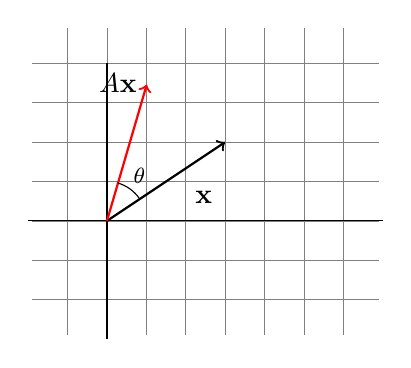
\begin{tikzpicture}[x=0.5cm, y=0.5cm]

\draw[step=0.5cm, style=help lines] (-1.9,-2.9) grid (6.9,4.9);
\draw (-2,0) -- (7,0);
\draw (0,-3) -- (0,4);

\draw[thick,->] (0,0) -- (3,2);
\draw (2,1) node[below right] {\Mtx{x}};

\draw[thick,red,->] (0,0) -- (1.01,3.46);
\draw (1,3) node[above left] {$A\Mtx{x}$};

\draw (0,0) +(34:0.5cm) arc (34:74:0.5cm);
\path (0,0) ++(54:0.7cm) node[font=\footnotesize] {$\theta$};

%\draw (1.5,1) arc (34:74:1cm);
%\path (0,0) ++(55:1.1cm) node[font=\footnotesize] {$\theta$};

\end{tikzpicture}

\end{center}


\end{frame}
%===========================================================

%===========================================================
\begin{frame}
  \frametitle{Linear dependence/independence}

\begin{itemize}
\item You'll remember that a \emph{linear combination} of vectors is an equation of the form $z = b_1 \Mtx{x}_1 + b_2 \Mtx{x}_2 + \cdots + b_p \Mtx{x}_p$

\item A list of vectors, $\Mtx{x}_1, \Mtx{x}_2, ..., \Mtx{x}_p$ , is said the be \emph{\textbf{linearly dependent}} if there is a non-trivial combination of them which ie qual to the zero vector.
\[
 b_1 \Mtx{x}_1 + b_2 \Mtx{x}_2 + \cdots + b_p \Mtx{x}_p = 0
\]

\item A list of vectors that are not linearly dependent are said to be \emph{\textbf{linearly independent}} 

\end{itemize}

\end{frame}
%===========================================================

%===========================================================
\begin{frame}
  \frametitle{Matrix Inverses}

\begin{itemize}
\item If $A$ is a \emph{square matrix} and $C$ is a matrix of the same size where $AC = I$ and $CA=I$ than $C$ is the inverse of $A$ and we denote is \Inv{A}.

\[
A\Inv{A} = \Inv{A}A = I
\]


\item Rules for inverses:

\begin{itemize}
 \item Only square matrices are invertible
 \item A matrix for which we can find an inverse is called \emph{\textbf{invertible}} (non-singular)
 \item A matrix for which no inverse exists is \emph{\textbf{singular}} (non-invertible)
 \item If $A$ and $B$ are both invertible $p \times p$ matrices than $\Inv{(AB)} = \Inv{B} \Inv{A}$ (note change in order).
\end{itemize}
 
\end{itemize}

\begin{Highlight}
  If a matrix is invertible than it's columns form a linearly independent list of vectors!
\end{Highlight}

\end{frame}
%===========================================================

%===========================================================
\begin{frame}
  \frametitle{More facts about Matrix Inverses}

 \begin{itemize}
 \item Not every square matrix is invertible
 \item Every orthogonal matrix is invertible
 \item Any diagonal matrix, $A$, where the $a_{ii}$ are non-zero, is invertible
 \end{itemize}
 
\end{frame} 

%===========================================================
\begin{frame}
  \frametitle{Simultaneous Linear Equations}

\begin{itemize}

\item A set of simultaneous linear equations are equations like the following:
\begin{eqnarray*}
x_1 + 3x_2 + 2x_3 & = & 3\\
-x_1 + x_2 + 2x_3 & = & -2\\
2x_1 + 4x_2 -2x_3 & = & 10
\end{eqnarray*}


\item Simultaneous linear equations have either:

\begin{itemize}
 \item No solutions
 \item One solution
 \item Infinitely many solutions
\end{itemize}
 
\end{itemize}


\end{frame}
%===========================================================

%===========================================================
\begin{frame}
  \frametitle{Matrices and Simultaneous Linear Equations}

\begin{itemize}

\item Matrices can be used to represent and solve simultaneous linear equations. For example,
\begin{eqnarray*}
x_1 + 3x_2 + 2x_3 & = & 3\\
-x_1 + x_2 + 2x_3 & = & -2\\
2x_1 + 4x_2 -2x_3 & = & 10
\end{eqnarray*}

\medskip
Can be represented by the equation $A\Mtx{x} = \Mtx{h}$:

\[
\left[
\begin{array}{ccc}
1 & 3 & 2 \\
-1 & 1 & 2 \\
2 & 4 & -2 \\
\end{array}
\right]
\left[
\begin{array}{c}
x_1 \\ x_2 \\ x_3
\end{array}
\right]
=
\left[
\begin{array}{c}
3 \\ -2 \\ 10
\end{array}
\right]
\]


\item Solve this equation by pre-multiplying both sides of the equation by \Inv{A}.
\begin{eqnarray*}
\Inv{A} A \Mtx{x} & = &\Inv{A} \Mtx{h} \\
\Mtx{x} & = &  \Inv{A} \Mtx{h}
\end{eqnarray*}

\end{itemize}


\end{frame}
%===========================================================

%===========================================================
\begin{frame}
  \frametitle{Simultaneous Equations and Matrix Inverses}

\begin{itemize}
\item $A\Mtx{x} = \Mtx{h}$ has a unique solution iff $A$ is invertible.

\item If $A$ is a singular matrix than $A\Mtx{x} = \Mtx{h}$ either has no solution or infinitely many solutions.

\end{itemize}

\end{frame}


% %===========================================================
% \begin{frame}
%   \frametitle{Homework}
% 
% \begin{itemize}
% \item Reading
% 
% \begin{itemize}
%  \item Wickens, chapters 3 and 4.
%  \item Matloff, chapters 4 and 5
%  \item For a review of linear algebra concepts pertinent to todays lecture see Hamilton, chapters 3 - 6, 8, and 16.
% \end{itemize}
% 
% \item Programming exercises
% \begin{itemize}
% 	\item See handout
% \end{itemize}
% 
% 
% \end{itemize}
% 
% \end{frame}
% %===========================================================



\end{document}
